\chapter{Background}
In this section the intention of using different types of biological input data is explained and what potentially will be the occuring problems. Afterwards the discretization algorithms, which binarize the data of the biological settings are explained. Then the graphtheoretical background of a boolean network in terms of structural and dynamic manner is defined and explained. Inferred boolean network need to be assessed proving that the applied inference method is significant. This performance measurement is achieved by different scoring metrics described in the last part of this section.


\section{Biological Background}

Depending on the aim of a network inference the biological input data can be depicted by the interaction of proteins, genes or metabolic substances. The choice of the biological input decides about the information content and thus the structure of the input data for further network inference algorithms. Biological interactions can be observed at different levels of information integration of a cell (gene gene interaction, protein protein interaction and metabolic interaction). 
In general, a signal binds to a membran integrated receptor of the cell causing an activation of one or multiple target proteins inducing several signal transduction cascades (Figure 2.1). While the signal is transduced, it is amplified by enzymatic activities or inhibited by feedback pathways down the cascade. Finally transcription factors are activated by the input signal such that the expression of a target gene by generating \gls{mRNA} (messanger RiboNucleotide Acid) results in a protein. The resulting proteins influence the cell's survival by its profileration, induction of cell differentiation and apoptosis.


\begin{figure}[H]
%\setlength{\abovecaptionskip}{0pt}
\captionsetup{width=0.9\linewidth}
\centering
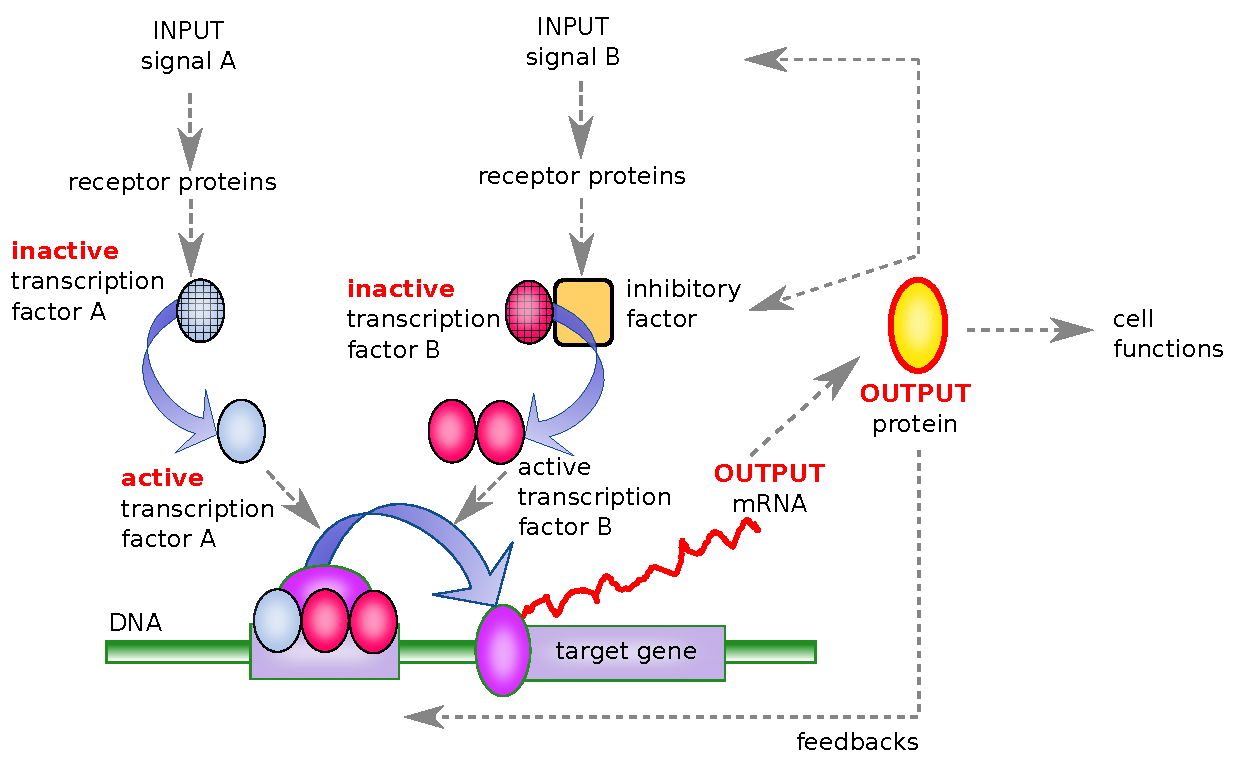
\includegraphics[width=0.9\textwidth]{./Bilder/GRN.pdf}
%\setlength{\abovecaptionskip}{-5ex}
\caption[Transcriptional Signale Cascade]{\textbf{Transcriptional Signale Cascade}
This example shows two different input signals $A$ and $B$ (e.g hormon) bind to specific receptor protein. The complex of $A$ activates the transcriptionfactor $A$ that binds directly to the gene's cis-regulatory sequence inducing the expression of the target gene.The complex of $B$ initiate a seperation of the inactive $B$ (pink oval) from an ihibitory factor (yellow rectangle). Transcription factor $B$ is then free to bind to the cis-regulatory sequence. Thus the expression level of this target gene is leveled by signal $A$ and $B$. The mRNA output results in a protein poduct which can be neccessary for cell functions, play a role in the gene transcription process or inluence the signal cascade of the input signals.
\citep{https://public.ornl.gov/site/gallery/detail.cfm?id=302&topic=&citation=&general=gene20regulatory20network&restsection=all} }
%\setlength{\belowcaptionskip}{0pt} 
\label{fig:Fig.2.}
\end{figure}


The concentration of substances in signalling pathways underlies high fluctuation over time due to transcriptional and translational regulation, such that the inference of a significant network is a challenging task.%\citep{BIES:BIES20834} \citep{https://www.ncbi.nlm.nih.gov/pmc/articles/PMC3436851/}.


\subsection*{Gene Regulatory Networks}

In a Gene regulatory network (\gls{GRN}) the interaction of genes are identified indirectly by the interaction and amount of thier transcriptional products (e.g. mRNA, proteins). %\citep{Modelling and analysis of gene regulatory networks}
The nodes of a GRN are depicted by the genes and the edges are directed by showing whether a gene produces mRNA (transcript of the source gene) which inhibits or activtes the target gene. %\citep{https://www.nature.com/articles/nrm2503}.


\subsection*{Metabolic networks}

At the level of Metabolic networks the substances are highly interconnected in a quite complex way (e.g. cell respiration in Figure 2.2). An indiviual's metabolism is determined by its genetics, enviroment and nutrition.\citep{8}. In a metabolic Network the nodes are depited by different biochemical components connected by directed edges describing the positive or negative interaction. Biochemical reaction are represented by a metabolic pathway, which consists of a sequence of biochemical reactions that produce a set of metabolites from a set of precursor metabolites and cofactors. The length of a pathway is the number of biochemical reactions between the precursor and the final metabolites of the pathway. The definition of a pathwy is not unique, therefore the length of pathways vary. \citep{9}

\begin{figure}[H]
\centering
\captionsetup{width=.8\linewidth}
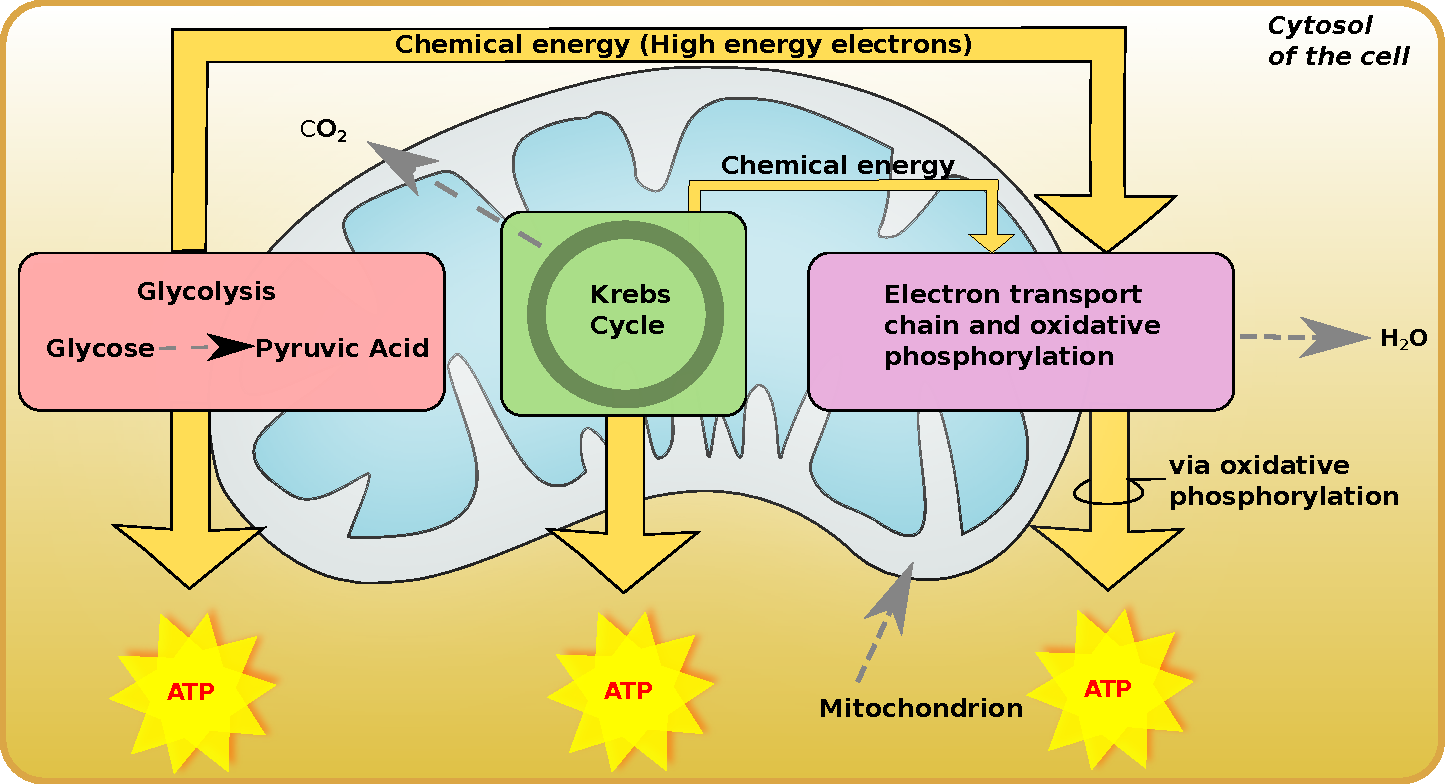
\includegraphics[width=0.8\textwidth]{./Bilder/metabolic.pdf}
\caption[Metabolic Network]{\textbf{Metabolic Network of the cell respiration. } Cell respiration in a mitochondrion, an essentiell compartment of the cell converting biochemnical energy from nutritiens into adenosin triphosphate (\gls{ATP}) by releasing waste products of water $H_{2}O$ and $CO_{2}$.}
\label{fig:Fig.3.}
\end{figure} 

\subsection*{Protein-Protein-Interaction network}
In contrast to the gene regulatory interaction network in a protein-protein interaction (\gls{PPI}) network the proteins act directly among themselve. Thus the nodes in a network are the interacting proteins. Proteins interact by physical contacts(e.g. electrostatic forces) of high specificity. PPIs play a big role in electron transfer,signal transduction, transport across membranes and cell metabolism. The underlying assumption is that true interactions are likely to occur between proteins involved in the same biological process, proteins found in the same cell compartment, and proteins whose mRNA are coexpressed.
%\citep{10.1371/journal.pcbi.1000807}
\citep{doi:10.1586/14789450.1.2.239}\\
The real-life data set of the Dream8 Challenge in this work is dealing with PPIs, thus, it is important to know for later data collection, data processing and discussion how the data is obtained and which role these PPIs play in the biological context.


\begin{figure}[H]
%\setlength{\abovecaptionskip}{0pt}
\captionsetup{width=.9\linewidth}
\centering
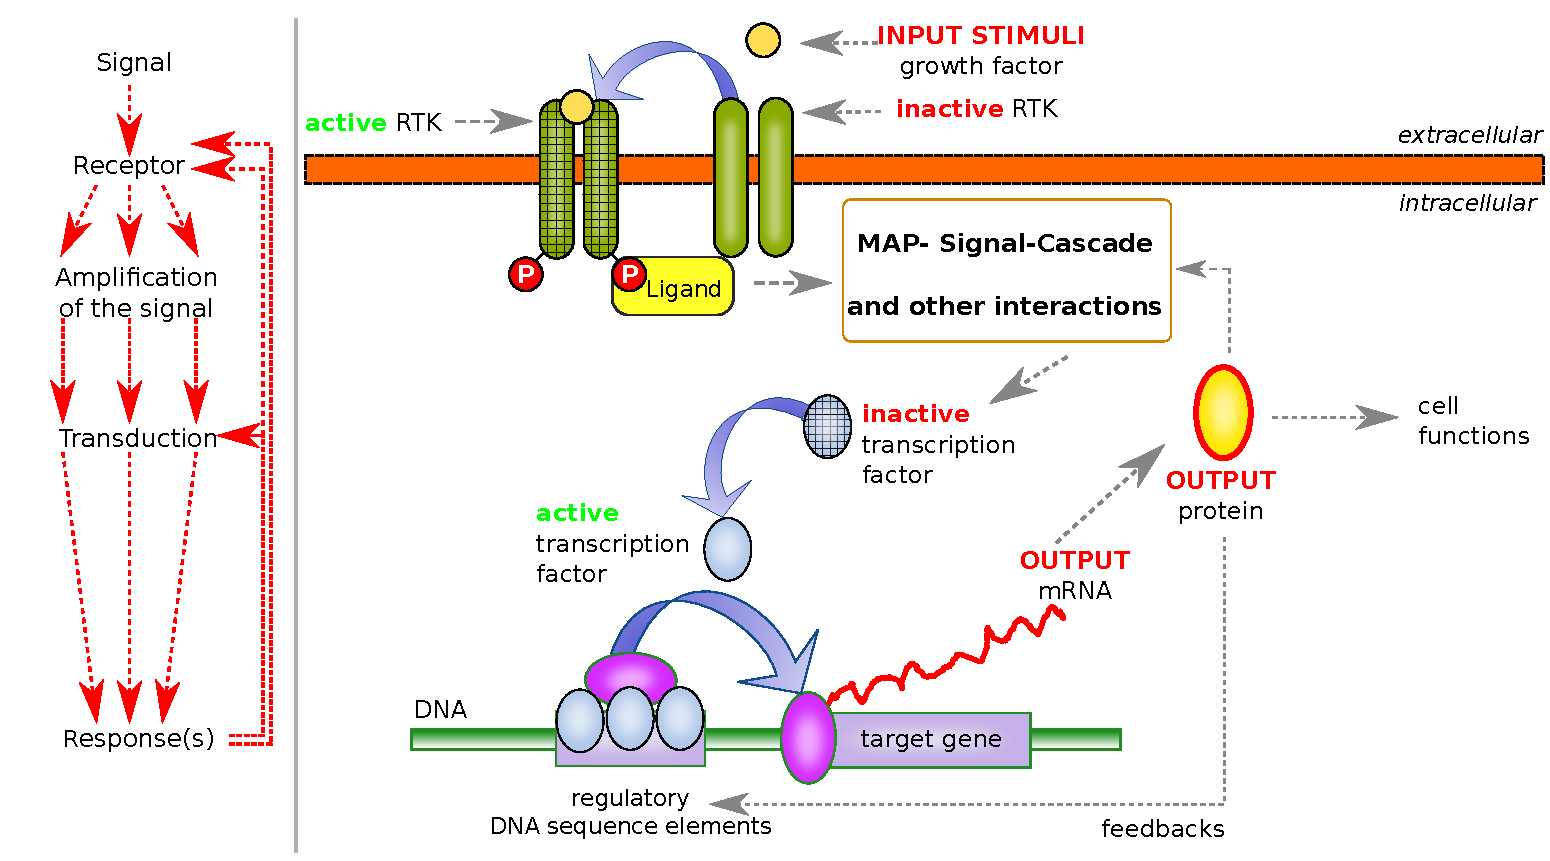
\includegraphics[width=0.9\textwidth]{./Bilder/GRNDREAM8.pdf}
%\setlength{\abovecaptionskip}{-5ex}
\caption[Transcriptional Signale Cascade of RTKs]{\textbf{Transcriptional Signale Cascade} An incoming stimuli (yellow circle) depicted as a growth factor binds to an inactive RTK (green), such that the RTK is activated. The RTK amplifies the signal and iniiates a signal transduction cascade, such that an inactive transcription fractor (blue oval) is activated, which binds to regulatory DNA sequence elements inducing the mRNA transcription of a target gene resulting in a new protein. The new protein can take place in cell functions or in the signal cascade. \citep{https://public.ornl.gov/site/gallery/detail.cfm?id=302&topic=&citation=&general=gene20regulatory20network&restsection=all} }
%\setlength{\belowcaptionskip}{0pt} 
\label{fig:DREAM8GRN}
\end{figure}

Referring to the general description of a transcriptional signal cascade (Figure 2.1) we state the receptor being an enzyme-associated receptor and the input signals are growth factors. A enzyme associated receptor has a polypetide chain integrated in the cell's membrane with a tyrosine kinase activity (Figure 2.3). Growthfactor receptors with a tyrosine kinase activity are called receptor tyrosine kinases (\gls{RTK}s). These RTKs have the property of autophosphorylation (resp. they amplify their incoming signal). Binds a ligand to this receptor, first the receptor autophosphorylates and then phosphorylates the tyrosin residues of the ligand. By the phosphorylation of the receptor and several other ligands (rep. proteins) a phosphorylating cascade (e.g. signal transduction cascade) is induced. In this Mitogen activated protein phosphorylation cascade the MAP-kinase katalyzes the phosphorylation of effector proteins, such that inactive transcription factors are activated starting the transcription process of a target gene and finally resulting in a protein.
%Quelle: Biochemie:Eine Einführung für Mediziner und Naturwissenschaftler, Werner Müller Esterl, 2009
For the Dream8 Challenge growth factors were selected depicted as stimuli by pertubating the cell's signal transduction. Thus, different stimuli cause different signal transduction cascades. Depending on the incoming stimuli particular proteins appear and take place in the signal transduction cascade. The goal is figure out the protein- protein interaction in this  phosphorylation cascade by inferring a boolean network based on the measurement of the proteins abundance considering different incoming growth factor (resp. stimuli) displayed in Table 2.1.


%{\tabcolsep=2.5pt%
\begin{center}
\captionsetup{width=0.87\linewidth}
%\setlength\extrarowheight{4pt}
%\noindent\begin{tabular}{c|c|l}
%\def\arraystretch{2.0}%
\scriptsize
%\addtolength{\tabcolsep}{-5pt}
\begin{tabular}{lll}
\toprule 
 Notation & Name & Description\\
\hline\hline
IGF1 & Insulin like Growth Factor 1 & \parbox{8cm}{Hormone, similar to the insulin function and structure}\\
\midrule NRG1 & Neuregulin 1 & \parbox{8cm}{Membrane glycoprotein, mediating cell-cell signalling, critical role in growth and developement of the cell}\\
\midrule HGF & Hepatocyte Growth Factor & \parbox{8cm}{Regulate cell growth, cell mortility and morphogenesis} \\
\midrule FGF1 & Fibroblast Growth Factor 1 & \parbox{8cm}{Functions as a modifier of endothelial cell migration, proliferation and an angiogenic factor}\\
\midrule Insulin & Insulin & \parbox{8cm}{Mutations in this gene are associated with type II diabetes and susceptibility to insulin resistance}\\
\midrule EGF & Epidermal Growth Factor & \parbox{8cm}{This protein acts a potent mitogenic factor that plays an important role in the growth, proliferation and differentiation of numerous cell types.}\\
\midrule PBS & Translocator Protein (TSPO) &  \parbox{8cm}{Present mainly in the mitochondrial compartment of peripheral tissues. The protein is a key factor in the flow of cholesterol into mitochondria to permit the initiation of steroid hormone synthesis.}\\
\midrule Seerum & SRF & \parbox{8cm}{Member of the MADS box superfamily
of transcription factors}\\
\bottomrule
\end{tabular}
\captionof{table}{List of growth factors of Dream8 Challenge}
%List of growth factors (resp. hormons) used in the Dream8 Challenge. All of them take place in the regulation of the cell's functions. Malfunctioning of these signals may cause several diseases (e.g. cancer).}
\end{center}
%}
%Quellen: https://www.ncbi.nlm.nih.gov/gene/

The dysregulation of the genes of these growth factors have been linked to diseases such as cancer, schizophrenia, bipolar disorder and many more.
%quelle(https://www.ncbi.nlm.nih.gov/gene/3084)

\subsubsection*{Reverse phase Protein lysate MicroArray}
One of the most effetive strategy to collect data of protein-protein interaction is a technique so called Reverse phase protein lysate microarray(\gls{RPMA}, resp. RPPA). RPMA is an antibody-based assay that provides quanitative measurements of protein abundance.
\citep{the HPN DREAM consotium}
This technique is divided up into 6 parts. First starting with the sample collection. An inhibitor or stimulus in form of drugs is added to a set of cell lines at the same time and the cell lines are then processed at different time points. Secondly in the cell lyses step cell fragments are lysed with a cell lysis buffer to obtain high protein concentration. The choice of a buffer decides the quantity of proteins that can be lysed out of the cell. Afterwards cell lysed probes are diluted. In the Antibody screening the lysates are pooled and resolved by \gls{SDS-PAGE} 
% https://www.ncbi.nlm.nih.gov/pubmed/21337110
(Sodium Dodecyl Sulfate - Polyacrylamide Gel Electrophoresis) followed by western blotting on a nitrocellulose membrane. The membrane is cut into 4mmm strips. Each slide is probed with a different antibody, where a primary antibody is extended by a secondary antibody. For fluorometric detection primary and secondary antibody are diluted (Figure 2.4).

\begin{figure}[H]
	%\setlength{\abovecaptionskip}{0pt}
	\captionsetup{width=0.7\linewidth}
	\centering
	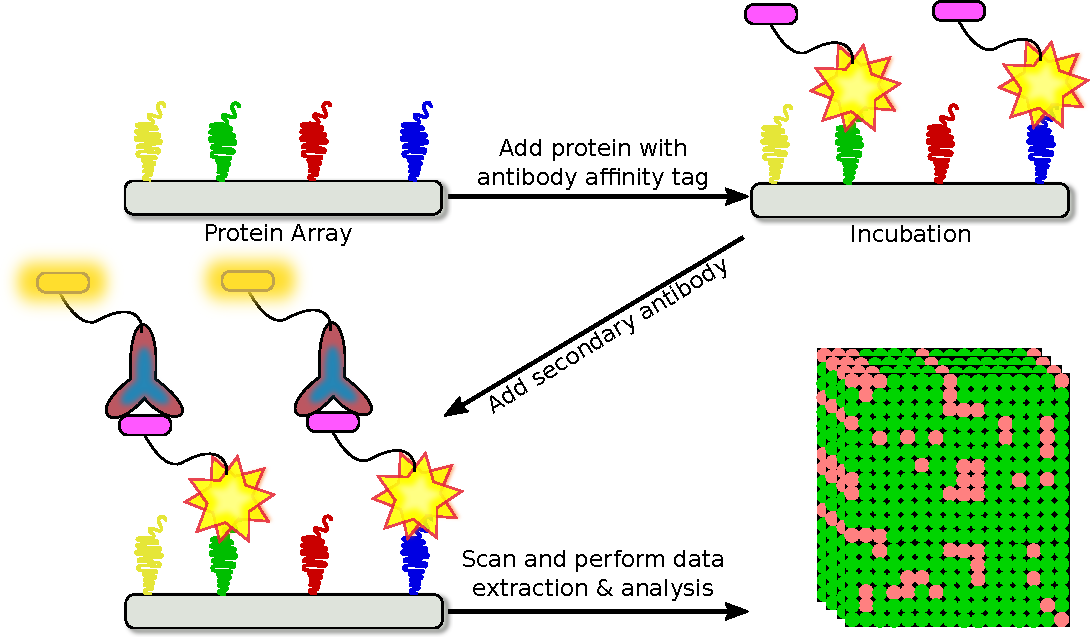
\includegraphics[width=0.7\textwidth]{./Bilder/RPMA.pdf}
	%\setlength{\abovecaptionskip}{-5ex}
	\caption[RPMA: Antibody binding and fluorometric detection]{\textbf{RPMA. Antibody binding and fluorometric detection.} Proteins are tagged by a specific antibody. After incubation time the secondary antibody is added. Finally the abundance of proteins is determined by a fluorometric detection.}
	%\setlength{\belowcaptionskip}{0pt} 
	\label{fig:Fig.4}
\end{figure}

A detection reagent is put on each slide. Signal amplification and detection is done by an optical flatbed scanner if colormetric technique is used or by laser scanning. The resulting data is normalized, such that outliers are excluded from the data's structure.\\

The strength of RPMA is the high throughput, ulta-sensitive detection of proteins from extremly small numbers of input material which is not possible for western blotting and \gls{ELISA} (Enzymatic Immunoassay). The small spot size on the microarray, ranging in diameter from 85 to 200 micrometres, enables the analysis of thousands of samples with the same antibody in one experiment. The high sensitivity of RPMA allows for the detection of low abundance proteins or biomarkers such as phosphorylated signaling proteins from very small amounts of starting material such as biopsy samples, which are often contaminated with normal tissue. A great improvement of RPMAs over traditional forward phase protein arrays is a reduction in the number of antibodies needed to detect a protein. The protein isn't detected directly which helps to preserve the proteins. Antibodies, especially phospho-specific reagents, often detect linear peptide sequences that may be masked due to the three-dimensional conformation of the protein. This problem is overcome with RPMAs as the samples can be denatured, revealing any covered epitopes (part of a protein recognized by specific antibody).\\

The weakness of RPMA are batch effects caused by the choice of the right buffer, quantity of the proteins and the antibody performance.
The choice of the right buffer decides the quantity of proteins which can be lysed out of the cell. Little or poor quality of starting material and a long storage time causes low protein. It might be useful to improve the antibody performance by validating it with a smaller sample size under identical conditions before starting with the actual sample collection. Currently the number of signaling proteins for which antibodies exist to get an analyzable signal is quite small. \\



\newpage
\section{Binarization Algorithms}
%normalization and discretization of the data
After generating the biological data some preprocessing like normalisation and discretization has to be done. Therefore several strategies are known. Normalization is an essential step, because data can contain outliers, the abundance of some proteins or mRNA is often higher than others and obtaining biological data from the lab could cause several batch effects. In section 3.3 Data collection of Dream8 Challenge data a normalization method is described.
Before starting inferring a boolean network from real-life time course data the data has to be discretisized (resp. binarized) such that each continous value (e.g. concentration measurement) measured at a certain time point of a particular substance (e.g. gene, protein) becomes discrete and has either a value of $1$ or $0$. This simplified representation of measurements decides about the significance of an inferred network. Therefore the choice of an appropriate binarization algorithm is necessary. Here two well known algorithms are introduced, the two clusters k-means binarization algorithm and the iterative k-means binarization algorithm.\\
The input of an inference problem, of a binarization algorithm respectively, consists of time course data $S=\{S_{1}, ...,S_{n}\}$ of $n$ species (e.g. genes, proteins), each of size $m+1$, where $S_{i}(t)\in\mathbb{R^{+}}$ $(0\le t \le m)$ is the concentration of species $i$ at time $t$. The binarization algorithms aim turning $S$ into a binary trajectory $B$ thus, a boolean network $N$ can be inferred from $B$.
%Quelle:TS2B Paper

\subsection*{Two clusters k-means binarization}
Given a set of time course data $S=\{S_{1}, ...,S_{n}\}$, where each observation $S_{i}(t)\in\mathbb{R^{+}}$ $(0\le t \le m)$ is a d-dimensional real vector, two k-means binarization aims to partition the $n$ observations into $k$ $(=2)$ cluster $C=\{C_{1},C_{2}\}$ by setting an obervation's value $S_{i}(t)$ to $1$ if it is above the overall mean $\mu(S)$ and setting to $0$ if an observation's value $S_{i}(t)$ is below (2.1).

\begin{equation}
\text{Two clusters k-means }=\begin{cases}
1 & \text{, if }S_{i}(t)\ge \mu (S)\\
0 & \text{, if }S_{i}(t)\le \mu (S)
\end{cases}
\end{equation}

%Quelle: TS2B Paper[11]
This binarization strategy is fast and simple but may exclude some essential information like about oscillations and fluctuations in a system (e.g. cell cycle). Therefore the interative k-means binarization method is introduced.
%\citep{10.1371/journal.pone.0066031}
%Shortly explain the meaning of oscillations



\subsection*{Iterative k-means binarization}

An initial depth $d$ of clustering is set followed by a set of initial number of cluster $k=2^d$. Then the method is divided up into two parts:

\begin{itemize}
\item[(1)] In each iteration the data of each species $S_{i}$  is classified into $k$ dijoint clusters $ C_{S{_i}}^{1},...C_{S{_i}}^{x}$. In each Cluster all its values are replacd by the clusters mean $\mu(C_{s_{i}}^{x})$.
\item[(2)]  In the next iteration step $d$ is decremeted by one and the clustering is repeated.
\end{itemize}

This iteration continues until $d=1$, where the data in the cluster with lower values of the mean are replaced by $0$ and higher values are replaced by $1$.


%Vllt. nochmal schauen ob es bessere mathematische Definition gibt?

\begin{exmp}Assume we have a time-series data with measurements for a gene $A$. Starting with a depth of $d=3$ we have initally $k=8$ clusters for each gene in the data set. This results in eight cluster $\{C_{s{_A}}^{1},...,C_{s{_A}}^{8}\}$ containing the time course data of gene $A$. Now for each cluster the mean $\{\mu(C_{s_{A}}^{1}),...,\mu(C_{s_{A}}^{8})\}$ is calculated. Afterwards values in each cluster are replaced by its mean. This is done 2 times more by decrementing $d$, such that $d=1$ and all values of $A$ being higher the overall mean are set to $1$ the one lower are set to $0$. \end{exmp}
%In the Diss. von Hannes Diskretisierungsstrategien anschauen
%siehe wiki: k-means for further discretization algorithms
%For d=1 beide methoden sind identisch!Überprüfen!



\newpage
\section{Graphtheoretical Background}
In this section the knowledge of the discretisized biological data is put into a graphtheoretical context of a boolean network.
%Define Boolean Network, describe Definition, give an example
\begin{defn}
\textbf{Undirected Graph and Directed Graph}\\
\textit{In general, an undirected graph $G=(V,E)$ is defined as a set of vertices $V$ describing the nodes of the system and a set of undirected edges $E = \{ (i,j)|i,j\in V\} $ that define a relationship between node $i$ and $j$. While in a \textbf{directed graph} $G=(V,A)$ is an ordered pair, defined as a set of vertices $V$ (nodes) and a set of directed edges $A$ (arcs). A set of directed edges $A=\{ (i,j)|\in V\} $ describes the flow of information in network, where $(i,j)$ describes the flow from $i$ (tail)to $j$ (head).}\\
\end{defn} 


%\begin{SCfigure}[][!h]
\begin{figure}[H]
%\begin{minipage}{0.5\linewidth}
%\vspace{-\baselineskip}
\vspace{-20px}
\centering
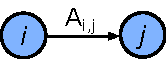
\includegraphics{./Bilder/DirectedGraph.pdf}
%\end{minipage}
\caption[Directed Graph]{\textbf{Directed Graph \textit{G}. } }
\label{fig:7}
%\end{SCfigure}
\end{figure}




\begin{defn}
\textbf{Boolean Network}\\
\textit{A boolean network is a directed graph $G(X,F)$, defined by a set of nodes $X$ in a binary vector $X(t)=\{x_{1}(t),...,x_{n}(t)\}$ representing state of a system at time $t$. Each element $x_{i}\in X$
corresponds to the state $x_{i}=1$ or $x_{i}=0$ of a species $i$. A set $F=\{f_{1},...,f_{n}\}$ of $n$ transition functions (resp.: set of boolean transition functions $B=\{f_{1},...f_{n}\}$) contains a particular function for each $x_{i}$. Every transition function $f_{i} \in F$ is therefore a n-variable Boolean function $f:\mathbb{B}^{n} \leftarrow \mathbb{B} $ which we can represent by a Boolean expression over $n$ input variables. %\citep{Klarner2015ContributionsTT}
\\For every $f_{i}\in F$ s.t. $1\le i\le n$,
\begin{center}$f_{i}(X(t))=x_{i}(t+1)$\end{center}
, where $f_{i}(X(t))$ defines the next state of $x_{i}$ at time $t$ in the network.}
\end{defn}

A Boolean network model is a directed graph whose nodes represent the elements of a system, edges represent orientation of regulatory relationships between elements, and every node can have two possible initial states $x_{i}\in \{0,1\}$ describing its activity [12-14].
%\citep{10.1371/journal.pone.0066031}
%Quelle: [TS2B-Paper]+davon die Quellen[12][14]
%\citep{Klarner2015ContributionsTT}
The activity of a node means a qualtative rate a gene is being transcribed $x_{i}=1$ or not $x_{i}=0$, a transcription factor is active oder inactive, a protein's concentration is above or below a certain threshold (e.g. phosporylated or un-phosphorylated). Thus a network with $n$ nodes will have $2^{n}$ possible states. As time passes the state of each node is determined by the states of its neighbors, through a rule called a transition function. In a boolean context the transition function is depicted as a boolean function determining the future state of a node. This boolean function is represented by logical operators 'NOT', 'AND' and 'OR' (resp. '\&\&', '||', '!' ;resp. '$\land$' ,'$\lor$' , '$\neg$'). \\
For instance a gene $x_{A}$ could be influenced by another gene $x_{B}$ positive and by a second gene $x_{C}$ negative (2.2). Then the boolean algebra would look like this:
\hspace{-10px}
\begin{equation}
\begin{split}
x_{A}& =x_{B} \text{ AND NOT } x_{C} \\
x_{A}& = x_{B} \text{ \&\&  !} x_{C} \\
x_{A}& = x_{B} \land \neg x_{C} 
\end{split}
\end{equation}

The application of the boolean function to a node's state returns a True or False state. Depending on the output of the boolean function, the state of the node either stays the same or changes. 
%Quelle: https://www.ncbi.nlm.nih.gov/pmc/articles/PMC2603008/)
%Quelle: [TS2B-Paper]+davon die Quellen[12][14]
\\
A boolean network is abstracted to a interaction graph covering the structural organization of a network, thus an interaction graph captures the dependencies between the variables and not the dynamics of a system.

\begin{defn}\textbf{Interaction Graph}\\
\textit{The interaction graph (\gls{IG}) of a boolean network $G(X,F)$ is a directed graph $IG(X,\rightarrow)$ that consists of the node set $X$ and the arc set $\leftarrow = \leftarrow _{F} \subseteq X \times X$ with $(x_{i},x_{j})\in \rightarrow \text{ iff }f_{x_{j}}$ depends on $x_{i}$ }
\end{defn} 
%\citep{Klarner2015ContributionsTT}
%Bespiel zeigen

In an interaction graph for each node being described by another one, this connection is written $x_{i}\rightarrow x_{j}$ (resp. $x_{i}$ $1$ $x_{j}$) and for the case that there is no connection $x_{i}\nrightarrow x_{j}$ (resp. $x_{i}$ $0$ $x_{j}$), respectively.
Another characteristic of interactions is wether they are activating or inhibiting or both depicted by the \textit{Sign} of an edge. 

\begin{defn}\textbf{\textit{Sign} of an edge}\\
\textit{The Sign of an edge is defined by $Sign(x_{i}\rightarrow x_{j} \subseteq \{+,-\})$.}
\end{defn}

Then the expression $x_{i}\rightarrow x_{j}$ is either $x_{i}\xrightarrow{+}  x_{j}$ (resp. $x_{i}$ $1$ $x_{j}$) describing an activating connection, $x_{i}\xrightarrow{-} x_{j}$ (resp. $x_{i}$ $-1$ $x_{j}$ ) describing an inhibitory connection or both $x_{i}\xrightarrow{+,-} x_{j}$ (resp. $x_{i}$ $1,-1$ $x_{j}$ ).\\


The \textbf{in-degree} of a node describes the number of incoming edges determining the node's state. Hence the outdegree describes the number of outgoing edges of a node. The in-degree is a major aspect of representing the complexity in a system, thus of the inference problem and plays a major role in centrality analysis in a network (Example 2.7).
%\citep{10.1371/journal.pone.0171097}
Nodes with only outcoing edges (in-degree$=0$) are called sources,and nodes with only incoming edges (out-degree$=0$) are sinks of the network. It is desireable to determine the nodes whos degree is the highest among other nodes, whose removal can break down the network into isolated clusters.\\
%\citep{RevModPhys.74.47}
%\begin{defn}\textbf{Indegree}\\
%\textit{}
%\end{defn}

Furthermore the dynamics of a system can be simulated by repeatedly applying all the transition functions to their variables and updating their states. This computation leads from an Interaction Graph to a State Tansition Graph.%\citep{SAADATPOUR20133}

\begin{defn}\textbf{State Transition Graph}\\
\textit{A State Transition Graph (\gls{STG}), where $STG(X,\rightarrow )$ is a directed graph with a set of nodes represented by a set of binary vectors $F(t+1)=\{ f_{1}(X(t+1)),...,f_{n}(X(t+1))\} $ representing the updated states of all variables after all of the functions in $F$ have executed. The arcs denote possible transitions from one binary state vector to another. }
\end{defn}%\citep{doi: https://doi.org/10.1016/j.ymeth.2012.10.012}\citep{Lee799}.\citep{Klarner2015ContributionsTT}
%\raggedbottom
The State TransitionGraph is either updated \textit{synchronously}, where each variable's state is updated simultaniously after all of the transition functions in $F$ have executed or \textit{asynchronously}, where the states are updated one at randomly choosing a transition function $f_{i}\in F$ and updating the state of $x_{i}$ immediatly. In biological processes interaction of substances rarely happen at the same time, thus dynamical analysis is an important factor of detecting interacting sustances.
\\\\
The following example shows how an interaction Graph looks like, how the transition functions (resp.boolean rules) are derived from this graph and how the State Transition Graph is constructed for the synchronous and asynchronous case.

\begin{exmp}
The interaction Graph in Figure 2.6 shows a boolean network with three nodes $X=\{x_{1},x_{2},x_{3}\}$ (blue circle), where positve (resp. activating) edges (green) and negative (resp. inhibiting) edges (red) represent the interaction between the nodes. The in-degree of $x_{1}=2$, $x_{2}=1$ and $x_{3}=3$.
\end{exmp}
 

\begin{figure}[!h]
%\begin{minipage}{0.4\linewidth}
%\vspace{-\baselineskip}
\centering
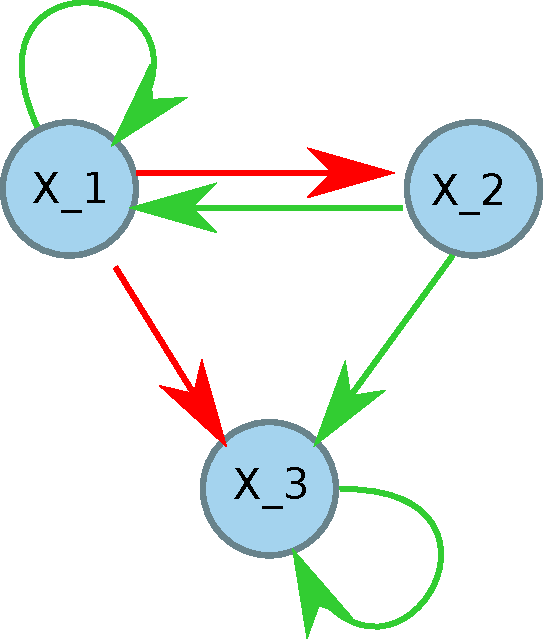
\includegraphics[scale=1.2]{./Bilder/examplenetwork.pdf}
%\end{minipage}
\caption[Interaction Graph]{\textbf{Interaction Graph}}
\label{fig:7}
\end{figure}
%\citep{Pipeline}
%Graphik und caption an die Breite der seite anpassen
%Caption text soll unter der Figure-Bezeichnung stehen.




From the interaction graph the set of transition functions $F$ (resp. boolean functions) can be derived (2.3) such that the state transition graph can be calculated.

\begin{equation}
f(x_{1,2,3}) = 
\begin{pmatrix}
x_1      & \land & x_2 & \land &\neg x_3\\
\neg x_1 &       &      &       & \\
         &       & x_2  &\land & x_3
\end{pmatrix}
\end{equation}


For every possible state of $x_i\in X$ the next state $f_{i}(X(t))=x_{i}(t+1)$ is calculated shown in the computation (2.4)-(2.11) below. This computation provide the new states for a synchronously updated state interaction graph displayed in the left graph in Figure 2.7.\citep{REMY2008335}


\begin{align}
x(t)& =(0,0,0) &\rightarrow & &f(x(t+1)) = (0,1,0)\\
\color{red}x(t)& \color{red}=(0,0,1) &\color{red}\rightarrow & &\color{red}f(x(t+1)) = (0,1,0)\\
x(t)& =(0,1,0) &\rightarrow & &f(x(t+1)) = (0,1,0)\\
x(t)& =(1,0,0) &\rightarrow & &f(x(t+1)) = (0,0,0)\\
x(t)& =(1,1,0) &\rightarrow & &f(x(t+1)) = (1,0,0)\\
\color{red}x(t)& \color{red}=(1,0,1) &\color{red}\rightarrow & &\color{red}f(x(t+1)) = (0,0,0)\\
x(t)& =(0,1,1) &\rightarrow & &f(x(t+1)) = (0,1,1)\\
\color{red}x(t)& \color{red}=(1,1,1) &\color{red}\rightarrow & &\color{red}f(x(t+1)) = (0,0,1)
\end{align}

The asynchronous updated state transition graph is computed by adding intermediate computation steps to the synchronus computation. Therefore the red highlighted computations (2.5),(2.9) and (2.11) are split by the amount of state changes. For instance in the computation step (2.5) $x(t)=(0,0,1)$ has two updates of states, $x_2$ changes and $x_3$ changes, too. As we know from the descriptin of asynchronous STG's in biological systems processes happen uncommonly at the same time. Thus the initial state $x(t)=(0,0,1)$ provides two possible updates: $f(x(t+1))=(0,1,1)$ and $f(x(t+1))=(0,0,0)$. The same procedure is done with (2.9) and (2.11) and finally the asynchronous STG can be drawn, shown by the right graph in Figure 2.7. 

\begin{figure}[h]
  \centering
 \begin{varwidth}{\linewidth}
    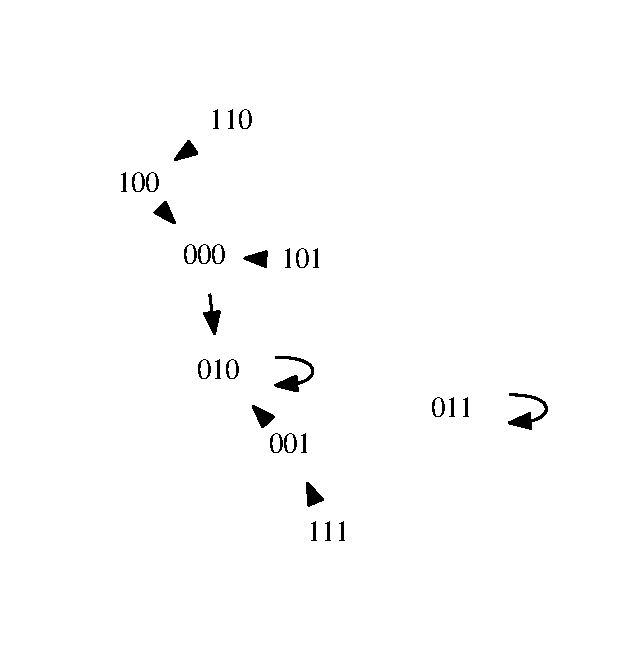
\includegraphics[scale=.7]{./Bilder/example01_synchron_stg}
  \end{varwidth} % ein Leerzeichen Abstand
  \begin{varwidth}{\linewidth}
    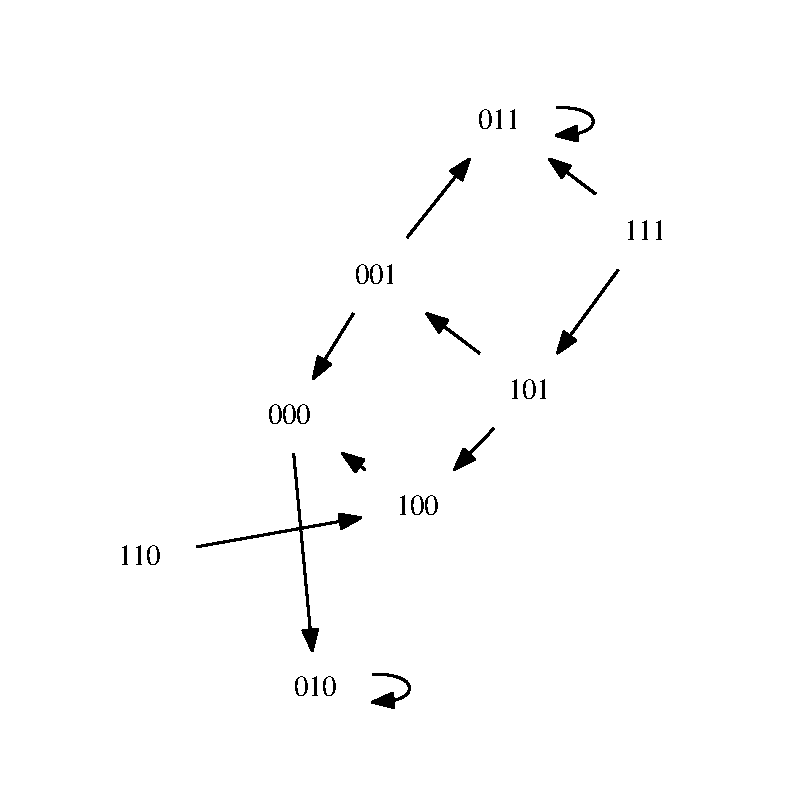
\includegraphics[scale=.6]{./Bilder/example01_asynchron_stg}
  \end{varwidth}
  \caption[Synchronous and Asynchronous State Transition Graph]{\textbf{Synchronous and Asynchronous State Transition Graph}. Left: Synchronous State Transition Graph; Right: Asynchronous State Transition Graph}
\label{fig:Fig.4.}
\end{figure}
%Mit inkscape schönermachen: beide .pdf zusammenfassen, mit Trennlinie

%Hinzuschreiben wasman noch alles mit STG machen kann:
%-Strucuralanalysis\\
%- Centrality measurements\\
%-Network motifs\\
%- Attractor, Basin analysis\\!!!Wichitg beschreiben, was ein attractor ist.
%-Network reduction
%S (set of states),B(binarized boolean trajectories),k(indegree value),n(number of nodes),m(number of measurements) Begriffe einführen
%\\newpage
